\documentclass[Rapport/Playerside/GameController/GameController.tex]{subfiles}
\label{sec:playerside_GameController_design}
\begin{document}
\subsubsection{Softwaredesign}
I dette afsnit beskrives design for GameController klassen på PlayerSideApp. Denne klasse er controller klassen for PlayerSideApp og indeholder alt den logik, der skal til, for at de 3 boundary klasser RPI\_IF, CupSensor\_IF og CupLight\_IF fungerer i et samlet system.\\
Under designet af denne klasse følges sekvensdiagrammet og statediagram i \textbf{Arkitekturen} i afsnit \fullref{arch:sec:playersideapp_application_model} og bruges de funktioner, der er defineret i de forskellige boundary klasser.\\\\
En vigtig funktionalitet i gamecontrolleren er blinkefunktionen af CupLight. Her anvendes en timer i PSoC komponent kataloget. Denne komponent startes og stoppes i klassens Controller funktion. Når timeren startes, skal den interrupte hvert halve sekund. Her bliver funktionen interrupt\_blink brugt i dens ISR, der skal kontrollere hvornår de 6 LED'er skal blinke. Timer komponenten kan ses i figur \ref{fig:Timer}.
\begin{figure}[H]
    \centering 
    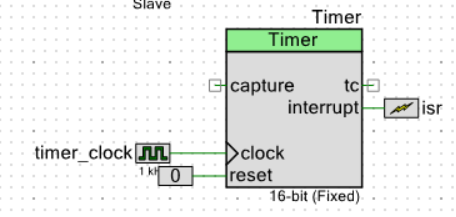
\includegraphics[width=0.5\linewidth]{Softwaredesign/GameController/graphic/gamecontroller_timer.PNG}
    \caption{Timer brugt til implementering af blink funktion}
    \label{fig:Timer}
\end{figure}
For en mere uddybende beskrivelse af design for GameController klassen, heri de forskellige funktioner, så se afsnit \fullref{swdesign:sec:GameController_design_bilag} i bilaget \textbf{Softwaredesign}.
\end{document}